%\section{正激波}
\begin{frame}{激波}
  \begin{columns}[c]
    \begin{column}{0.6\textwidth}
      \begin{itemize}[<+-|alert@+>]
        \item 在气流通过强压缩波时,气流受到突然的压缩,其压强、温度和密度等都将
          突跃地升高,而速度则突跃地降低。这种突跃变化的强压缩波称为
          {\color{blue}激波}
        \item 按照激波的形状,可将激波划分为:
      \end{itemize}
      \only<3>{
        \begin{enumerate}
          \item {\color{blue}正激波}。波面与气流方向相垂直的平面激波,气流通过薄面后,不改变流动方向
            \begin{center}
              \begin{tikzpicture}
                \draw[thick,red] (1, -1) -- (1, 1);
                \draw[-latex] (0,0) -- node[midway, above,anchor=south west]{$v_{1}$} (0.5,0);
                \draw[-latex] (1.5,0) -- node[midway, above,anchor=south west]{$v_{2}$} (2.0,0);
              \end{tikzpicture}
            \end{center}
        \end{enumerate}
      }
      \only<4>{
        \begin{enumerate}
          \setcounter{enumi}{1}
        \item {\color{blue}斜激波}。波面与气流方向不垂直的平面激波,气流通过波面后,要改变流动方向
          \begin{center}
            \begin{tikzpicture}
              \def\firstcircle{(1,0) circle (1.3cm)}
              \draw[thick,red] (1,0) -- ++(30:1.5);
              \draw[thick,red] (1,0) -- ++(-30:1.5);
              \begin{scope}
                \clip \firstcircle;
              \filldraw[thick,pattern=north east lines] (1, 0) -- (2.5, 0.4) -- (2.5, -0.4) -- cycle;
            \end{scope}
            \draw[-latex] (0,0) -- (0.5,0);
          \end{tikzpicture}
        \end{center}
    \end{enumerate}
  }
  \only<5>{
    \begin{enumerate}
      \setcounter{enumi}{2}
    \item {\color{blue}脱体激波}。波形是弯曲的,也称为曲激波。当超声速气流流过钝头物体时,物体的前面将产生脱体激波
      \begin{center}
        \begin{tikzpicture}
          \draw[-latex] (0,0) -- (0.5,0);
          \begin{scope}
            \clip (0.8,-1.3) rectangle (1.2, 1.3);
          \draw[thick, red] (5,0) circle (4cm);
        \end{scope}
        \begin{scope}
          \clip (1.5,0) circle (0.6);
        \filldraw[thick,pattern=north east lines] (2,0) ellipse (0.5cm and 0.3cm);
      \end{scope}
    \end{tikzpicture}
  \end{center}
          \end{enumerate}
        }
      \end{column}
      \begin{column}{0.4\textwidth}
        \begin{figure}
          \includegraphics[width=5cm]{img/shockwave.jpg}
        \end{figure}
      \end{column}
    \end{columns}
  \end{frame}

\subsection{激波的形成}
\begin{frame}{激波的形成}
  \begin{columns}[c]
    \begin{column}{0.4\textwidth}
  \vspace*{-1em}
  \begin{center}
  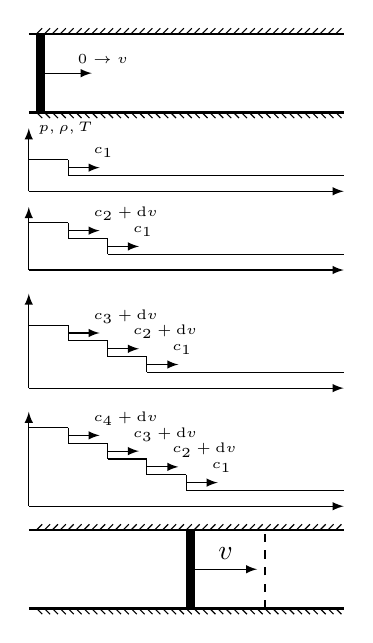
\begin{tikzpicture}
    \begin{scope}
      \draw[thick] (0,0) -- (4,0);
      \draw[thick] (0,1) -- (4,1);
      \draw[fill=black] (0.1,0) rectangle (0.2,1);
    \foreach \p in 
    {0.1, 0.2, 0.3, 0.4, 0.5, 0.6, 0.7, 0.8, 0.9, 1.0,
     1.1, 1.2, 1.3, 1.4, 1.5, 1.6, 1.7, 1.8, 1.9, 2.0,
     2.1, 2.2, 2.3, 2.4, 2.5, 2.6, 2.7, 2.8, 2.9, 3.0,
     3.1, 3.2, 3.3, 3.4, 3.5, 3.6, 3.7, 3.8, 3.9}
    {
      \draw[thin] (\p, 0) -- ++(-45:0.1);
      \draw[thin] (\p, 1) -- ++(45:0.1);
    }
    \draw[-latex] (0.2,0.5) -- node[pos=0.5,above,anchor=south west]{\tiny $0\rightarrow v$} (0.8,0.5);
    \end{scope}
    \begin{scope}[yshift=-1.0cm]
      \draw[-latex](0,0) -- (4,0);
      \draw[-latex](0,0) -- (0,0.8) node[right]{\tiny $p,\rho, T$};
      \draw (0,0.4) -- (0.5,0.4);
      \draw (0.5,0.4) -- (0.5,0.2);
      \draw[-latex] (0.5,0.3) -- node[midway,anchor=south west]{\tiny $c_{1}$}(0.9,0.3);
      \draw (0.5,0.2) -- (4,0.2);
    \end{scope}
    \begin{scope}[yshift=-2.0cm]
      \draw[-latex](0,0) -- (4,0);
      \draw[-latex](0,0) -- (0,0.8);
      \draw (0,0.6) -- (0.5,0.6);
      \draw (0.5,0.6) -- (0.5,0.4);
      \draw[-latex] (0.5,0.5) -- node[midway,anchor=south west]{\tiny $c_{2}+\mathrm{d}v$}(0.9,0.5);
      \draw (0.5,0.4) -- (1,0.4);
      \draw (1,0.4) -- (1,0.2);
      \draw[-latex] (1,0.3) -- node[midway,anchor=south west]{\tiny $c_{1}$}(1.4,0.3);
      \draw (1,0.2) -- (4,0.2);
    \end{scope}
    \begin{scope}[yshift=-3.5cm]
      \draw[-latex](0,0) -- (4,0);
      \draw[-latex](0,0) -- (0,1.2);
      \draw (0,0.8) -- (0.5,0.8);
      \draw (0.5,0.8) -- (0.5,0.6);
      \draw[-latex] (0.5,0.7) -- node[midway,anchor=south west]{\tiny $c_{3}+\mathrm{d}v$}(0.9,0.7);
      \draw (0.5,0.6) -- (1,0.6);
      \draw (1.0,0.6) -- (1,0.4);
      \draw[-latex] (1.0,0.5) -- node[midway,anchor=south west]{\tiny $c_{2}+\mathrm{d}v$}(1.4,0.5);
      \draw (1,0.4) -- (1.5,0.4);
      \draw (1.5,0.4) -- (1.5,0.2);
      \draw[-latex] (1.5,0.3) -- node[midway,anchor=south west]{\tiny $c_{1}$}(1.9,0.3);
      \draw (1.5,0.2) -- (4,0.2);
    \end{scope}
    \begin{scope}[yshift=-5.0cm]
      \draw[-latex](0,0) -- (4,0);
      \draw[-latex](0,0) -- (0,1.2);
      \draw (0,1) -- (0.5,1);
      \draw (0.5,1) -- (0.5,0.8);
      \draw[-latex] (0.5,0.9) -- node[midway,anchor=south west]{\tiny $c_{4}+\mathrm{d}v$}(0.9,0.9);
      \draw (0.5,0.8) -- (1,0.8);
      \draw (1,0.8) -- (1,0.6);
      \draw[-latex] (1,0.7) -- node[midway,anchor=south west]{\tiny $c_{3}+\mathrm{d}v$}(1.4,0.7);
      \draw (1,0.6) -- (1.5,0.6);
      \draw (1.5,0.6) -- (1.5,0.4);
      \draw[-latex] (1.5,0.5) -- node[midway,anchor=south west]{\tiny $c_{2}+\mathrm{d}v$}(1.9,0.5);
      \draw (1.5,0.4) -- (2,0.4);
      \draw (2.0,0.4) -- (2,0.2);
      \draw[-latex] (2,0.3) -- node[midway,anchor=south west]{\tiny$c_{1}$}(2.4,0.3);
      \draw (2.0,0.2) -- (4,0.2);
    \end{scope}
    \begin{scope}[yshift=-6.3cm]
      \draw[thick] (0,0) -- (4,0);
      \draw[thick] (0,1) -- (4,1);
      \draw[fill=black] (2,0) rectangle (2.1,1);
    \foreach \p in 
    {0.1, 0.2, 0.3, 0.4, 0.5, 0.6, 0.7, 0.8, 0.9, 1.0,
     1.1, 1.2, 1.3, 1.4, 1.5, 1.6, 1.7, 1.8, 1.9, 2.0,
     2.1, 2.2, 2.3, 2.4, 2.5, 2.6, 2.7, 2.8, 2.9, 3.0,
     3.1, 3.2, 3.3, 3.4, 3.5, 3.6, 3.7, 3.8, 3.9}
    {
      \draw[thin] (\p, 0) -- ++(-45:0.1);
      \draw[thin] (\p, 1) -- ++(45:0.1);
    }
    \draw[-latex] (2.1,0.5) -- node[midway,above]{$v$} (2.9,0.5);
    \draw[dashed] (3,0) -- (3,1);
    \end{scope}
  \end{tikzpicture}
  \end{center}
    \end{column}
  
    \begin{column}{0.6\textwidth}
    \only<2-4>{
\begin{itemize}[<+(1)->]
  \item 现有一个充满静止气体的长直圆管,管中有一活塞。该活塞向右作突然加速运动,其速度从零加速到某一速度$v$,之后以该速度作匀速运动。
  \item 把这个扰动过程分成无数个微小的阶段。每个微小阶段均是一个微弱压缩扰动。设
    每个微弱压缩扰动产生微小压强增量$\mathrm{d}p$,每个微小阶段活塞速度增加
    $\mathrm{d}v$
  \item 当活塞开始运动时,产生的第一个微弱扰动波以声速$c_{1}$传播,扰动后气体获得与活塞相同的速度$\mathrm{d}v$,压强为
    $p_{2}=p_{1}+\mathrm{d}p$,密度为$\rho_{2}=\rho_{1}+\mathrm{d}\rho$,温度为
    $T_{2}=T_{1}+\mathrm{d}T$
\end{itemize}
}
\only<5-7>{
  \begin{itemize}[<+(4)->]
  \item 紧接着产生第二个微弱扰动波,并在被第一个微弱扰动波扰动过的气体中传播。第
    二个微弱扰动波的声速$c_{2}=\sqrt{\gamma RT_{2}}$,波速为$c_{2}+\mathrm{d}v$
    。扰动后活塞速度又增加$\mathrm{d}v$,气体速度为$2\mathrm{d}v$,压强为
    $p_{3}=p_{2}+\mathrm{d}p$,密度为$\rho_{3}=\rho_{2}+\mathrm{d}\rho$,温度为
    $T_{3}=T_{2}+\mathrm{d}T$
  \item 接着第三个微弱扰动波产生,并在第二个微弱扰动波扰动过的气体中传播,依次类
    推
    \item $p_{1}<p_{2}<p_{3}<\cdots$,$\rho_{1}<\rho_{2}<\rho_{3}<\cdots$,$T_{1}<T_{2}<T_{3}<\cdots$,$c_{1}<c_{2}<c_{3}<\cdots$,$c_{1}<c_{2}+\mathrm{d}v<c_{3}+2\mathrm{d}v<\cdots$
\end{itemize}
}
\only<8-10>{
  \begin{itemize}[<+(7)->]
    \item 在整个活塞压缩过程中,管道内将产生并形成若干道微弱压缩波,每一个波的传播速度不一样,后一个时刻产生的微弱扰动波的传播速度将大于前一时刻产生的微弱扰动波的传播速度
    \item 经过一段时间后,后产生的微弱扰动波将逐渐接近先产生的微弱扰动波,波与波之间的距离逐渐缩小,波形越来越陡
    \item 最后,后面的波赶上前面的破,所有的微弱扰动波聚集在一起,叠加成一个垂直于流动方向的具有压强不连续面的强压缩波,即正激波
  \end{itemize}
}
\only<11->{
  \vspace*{-1em}
  \begin{itemize}[<+(10)->]
    \item 往后,随着活塞匀速$v$继续运动,管道内能维持一个强度不变的正激波
    \item 正激波后面受到扰动的气体,其速度由扰动前的零增加到与活塞相同的速度$v$
    \item 正激波传播速度大于未受扰动气体的声速$c_{1}$
    \item 正激波的这种突跃变化是不连续的,是在与气体分子平面自由程同一数量级内完
      成(空气约$3\times10^{-4}\mathrm{mm}$)
    \item 宏观上可以认为是在一个几何面上突然变化的,即激波是不连续的间断面,气流
      通过激波的变化是突然的、不连续的
  \end{itemize}
}
    \end{column}
    
  \end{columns}
\end{frame}

\subsection{正激波的基本方程}
\begin{frame}{正激波的基本方程}
  \vspace*{-1em}
  \begin{center}
  \begin{tikzpicture}
\begin{scope}
    \draw[thick] (0,0) -- (5,0);
    \draw[thick] (0,1.5) -- (5,1.5);
    %\draw[thick] (2,0) node[anchor=north]{$n$} -- (2,1.5) node[anchor=south]{$m$};
    \filldraw[thick,pattern=north east lines] (2.6,0) -- (2.6,1.5) -- (2.4,1.5)
      -- (2.4, 0) -- cycle;
    \draw[thick,-latex] (2.5,0.75) -- node[midway,above]{$v_{s}$} node[midway,below]{$p_{1}$}(3.5,0.75);
    \draw[thick,-latex] (1.0,0.75) -- node[midway,above]{$v_{g}$}
      node[midway,below]{$p_{2}$} (2.2,0.75);
    \foreach \p in 
    {0.1, 0.2, 0.3, 0.4, 0.5, 0.6, 0.7, 0.8, 0.9, 1.0,
     1.1, 1.2, 1.3, 1.4, 1.5, 1.6, 1.7, 1.8, 1.9, 2.0,
     2.1, 2.2, 2.3, 2.4, 2.5, 2.6, 2.7, 2.8, 2.9, 3.0,
     3.1, 3.2, 3.3, 3.4, 3.5, 3.6, 3.7, 3.8, 3.9, 4.0,
     4.1, 4.2, 4.3, 4.4, 4.5, 4.6, 4.7, 4.8, 4.9}
    {
      \draw[thin] (\p, 0) -- ++(-45:0.1);
      \draw[thin] (\p, 1.5) -- ++(45:0.1);
    }
  \end{scope}
  \begin{scope}[xshift=6cm]
    \draw[thick] (0,0) -- (5,0);
    \draw[thick] (0,1.5) -- (5,1.5);
    %\draw[thick] (2,0) node[anchor=north]{$n$} -- (2,1.5) node[anchor=south]{$m$};
    \filldraw[thick,pattern=north east lines] (2.6,0) -- (2.6,1.5) -- (2.4,1.5)
      -- (2.4, 0) -- cycle;
    \draw[dashed,thick] (2.3,0) node[below,anchor=north]{$2$} -- (2.3,1.5)
      node[above,anchor=south]{$2$};
    \draw[dashed,thick] (2.7,0) node[below,anchor=north]{$1$} -- (2.7,1.5)
      node[above,anchor=south]{$1$};
    \draw[thick,-latex] (2.0,0.75) -- node[midway,above]{$v_{2}=v_{s}-v_{g}$} node[midway,below]{$p_{2}$} (0.2,0.75);
    \draw[thick,-latex] (4.8,0.75) -- node[midway,above]{$v_{1}=v_{s}$} node[midway,below]{$p_{1}$}(3.0,0.75);
    \foreach \p in 
    {0.1, 0.2, 0.3, 0.4, 0.5, 0.6, 0.7, 0.8, 0.9, 1.0,
     1.1, 1.2, 1.3, 1.4, 1.5, 1.6, 1.7, 1.8, 1.9, 2.0,
     2.1, 2.2, 2.3, 2.4, 2.5, 2.6, 2.7, 2.8, 2.9, 3.0,
     3.1, 3.2, 3.3, 3.4, 3.5, 3.6, 3.7, 3.8, 3.9, 4.0,
     4.1, 4.2, 4.3, 4.4, 4.5, 4.6, 4.7, 4.8, 4.9}
    {
      \draw[thin] (\p, 0) -- ++(-45:0.1);
      \draw[thin] (\p, 1.5) -- ++(45:0.1);
    }
  \end{scope}
  \end{tikzpicture}
  \end{center}
  取激波两侧的1-1、2-2两个断面之间气流组成控制体。

  连续性方程:
  \begin{equation*}
    \rho_{1}v_{1}
    =
    \rho_{2}v_{2}
  \end{equation*}
  动量方程:
  \begin{equation*}
    p_{1}-p_{2}
    =
    \rho_{1}v_{1}(v_{2}-v_{1})
  \end{equation*}
  \begin{equation*}
    p_{1}
    +
    \rho_{1}v_{1}^{2}
    =
    p_{2}
    +
    \rho_{2}v_{2}^{2}
  \end{equation*}
  能量方程:
  \begin{equation*}
    h_{1}
    +
    \frac{v_{1}^{2}}{2}
    =
    h_{2}
    +
    \frac{v_{2}^{2}}{2}
  \end{equation*}
\end{frame}

\subsection{兰金-许贡纽公式}
\begin{frame}{兰金-许贡纽公式(Rankine-Hugoniot)}
  \vspace*{-1em}
  \begin{equation*}
    \rho_{1}v_{1}
    =
    \rho_{2}v_{2}
  \end{equation*}
  \begin{equation*}
    p_{1}-p_{2}
    =
    \rho_{1}v_{1}(v_{2}-v_{1})
  \end{equation*}
  \begin{equation*}
  v_{1}-v_{2}
  =
  \frac{p_{2}}{\rho_{2}v_{2}}
  -
  \frac{p_{1}}{\rho_{1}v_{1}}
  \quad\quad\quad
    v_{1}+v_{2}
    =
    \frac{\rho_{1}v_{1}}{\rho_{1}}
    +
    \frac{\rho_{2}v_{2}}{\rho_{2}}
  \end{equation*}
  \begin{equation*}
    \begin{aligned}
    v_{1}^{2}-v_{2}^{2}
    &=
    \left(
  \frac{p_{2}}{\rho_{2}v_{2}}
  -
  \frac{p_{1}}{\rho_{1}v_{1}}
    \right)
    \left(
    \frac{\rho_{1}v_{1}}{\rho_{1}}
    +
    \frac{\rho_{2}v_{2}}{\rho_{2}}
    \right)
    %两个括号内的分母和分子可以相互抵消
    \\
    &=
    (p_{2}-p_{1})
    \left(\frac{1}{\rho_{2}}+\frac{1}{\rho_{1}}\right)
    \end{aligned}
  \end{equation*}
  \begin{equation*}
    h_{1}
    +
    \frac{v_{1}^{2}}{2}
    =
    h_{2}
    +
    \frac{v_{2}^{2}}{2}
  \end{equation*}
  \begin{equation*}
    \tikzmarkin<2->[h2]{c7s5s1t1}
    h_{2}-h_{1}
    =
    \frac{1}{2}\left(\frac{1}{\rho_{2}}+\frac{1}{\rho_{1}}\right)
    (p_{2}-p_{1})
    \tikzmarkend{c7s5s1t1}
  \end{equation*}
    \onslide<2->{
    \begin{tikzpicture}[remember picture, overlay]
      \coordinate (c7s5s1t1-aa) at ($(c7s5s1t1)+(7.2,-0.25)$);
      \node[align=left,above,red] at (c7s5s1t1-aa) {\small 兰金-许贡纽公式};
      \path[-latex,red, draw] (c7s5s1t1-aa) |- ($(c7s5s1t1)+(5.75,-0.5)$);
    \end{tikzpicture}
  }
\end{frame}

\begin{frame}{压强突变与密度突变对应关系}
  \vspace*{-1.5em}
  \begin{equation*}
    h_{2}-h_{1}
    =
    \frac{1}{2}\left(\frac{1}{\rho_{2}}+\frac{1}{\rho_{1}}\right)
    (p_{2}-p_{1})
  \end{equation*}
 对于完全气体
 \vspace*{-1em}
 \begin{equation*}
 h
 =
 \frac{\gamma}{\gamma-1}\frac{p}{\rho}
 \end{equation*}
 \begin{equation*}
   \frac{\gamma}{\gamma-1}\frac{p_{2}}{\rho_{2}}
   -
   \frac{\gamma}{\gamma-1}\frac{p_{1}}{\rho_{1}}
   =
    \frac{1}{2}\left(\frac{1}{\rho_{2}}+\frac{1}{\rho_{1}}\right)
    (p_{2}-p_{1})
 \end{equation*}
 \only<2-5>{
   \begin{equation*}
   \frac{\gamma}{\gamma-1}
   \frac{p_{2}\rho_{1}-p_{1}\rho_{2}}{\rho_{1}\rho_{2}}
   =
   \frac{1}{2}
   \frac{\rho_{1}+\rho_{2}}{\rho_{1}\rho_{2}}(p_{2}-p_{1})
   \end{equation*}
 }
 \only<3-5>{
   \begin{equation*}
   \frac{\gamma}{\gamma-1}
 (p_{2}\rho_{1}-p_{1}\rho_{2})
   =
   \frac{1}{2}
   (\rho_{1}+\rho_{2})(p_{2}-p_{1})
   =
   \frac{1}{2}
   (p_{2}\rho_{1}-p_{1}\rho_{2})
   +
   \frac{1}{2}
   (p_{2}\rho_{2}-p_{1}\rho_{1})
   \end{equation*}
 }
 \only<4-5>{
   \begin{equation*}
     \frac{\gamma+1}{\gamma-1}(p_{2}\rho_{1}-p_{1}\rho_{2})
     =
     (p_{2}\rho_{2}-p_{1}\rho_{1})
   \end{equation*}
 }
 \only<5-6>{
   \begin{equation*}
   \frac{\gamma+1}{\gamma-1}
   \left(\frac{p_{2}}{p_{1}}-\frac{\rho_{2}}{\rho_{1}}\right)
   =
   \frac{p_{2}}{p_{1}}\frac{\rho_{2}}{\rho_{1}}-1
   \end{equation*}
 }
 \only<6>{
   \begin{equation*}
     \left(\frac{\gamma+1}{\gamma-1}-\frac{\rho_{2}}{\rho_{1}}\right)\frac{p_{2}}{p_{1}}
     =
     \frac{\gamma+1}{\gamma-1}\frac{\rho_{2}}{\rho_{1}}-1
   \end{equation*}
   \begin{equation*}
     \left(\frac{\gamma+1}{\gamma-1}+\frac{p_{2}}{p_{1}}\right)\frac{\rho_{2}}{\rho_{1}}
     =
     \frac{\gamma+1}{\gamma-1}\frac{p_{2}}{p_{1}}+1
   \end{equation*}
 }
 \uncover<7->{
 \begin{equation*}
   \frac{\rho_{2}}{\rho_{1}}
   =
   \dfrac
   {\dfrac{\gamma+1}{\gamma-1}\dfrac{p_{2}}{p_{1}}+1}
   {\dfrac{\gamma+1}{\gamma-1}+\dfrac{p_{2}}{p_{1}}}
   \quad
   \mbox{或}
   \quad
   \frac{p_{2}}{p_{1}}
   =
   \dfrac
   {\dfrac{\gamma+1}{\gamma-1}\dfrac{\rho_{2}}{\rho_{1}}-1}
   {\dfrac{\gamma+1}{\gamma-1}-\dfrac{\rho_{2}}{\rho_{1}}}
 \end{equation*}
 }
 \uncover<8->{
 \begin{equation*}
   \frac{T_{2}}{T_{1}}
   =
   \frac{p_{2}}{p_{1}}
   \frac{\rho_{1}}{\rho_{2}}
   =
   \frac{p_{2}}{p_{1}}
   \dfrac
   {\dfrac{\gamma+1}{\gamma-1}+\dfrac{p_{2}}{p_{1}}}
   {\dfrac{\gamma+1}{\gamma-1}\dfrac{p_{2}}{p_{1}}+1}
   =
   \dfrac
   {\dfrac{\gamma+1}{\gamma-1}\dfrac{p_{2}}{p_{1}}+\left(\dfrac{p_{2}}{p_{1}}\right)^{2}}
   {\dfrac{\gamma+1}{\gamma-1}\dfrac{p_{2}}{p_{1}}+1}
 \end{equation*}
 }
\end{frame}

\begin{frame}{压强突变与密度突变对应关系图}
  \begin{columns}[c]
    \begin{column}{0.4\textwidth}
      \vspace*{-1em}
 \begin{equation*}
   \begin{aligned}
   \frac{p_{2}}{p_{1}}
   &=
   \dfrac
   {\dfrac{\gamma+1}{\gamma-1}\dfrac{\rho_{2}}{\rho_{1}}-1}
   {\dfrac{\gamma+1}{\gamma-1}-\dfrac{\rho_{2}}{\rho_{1}}}
   \\
   \frac{T_{2}}{T_{1}}
   &=
   \dfrac
   {\dfrac{\gamma+1}{\gamma-1}\dfrac{p_{2}}{p_{1}}+\left(\dfrac{p_{2}}{p_{1}}\right)^{2}}
   {\dfrac{\gamma+1}{\gamma-1}\dfrac{p_{2}}{p_{1}}+1}
   \end{aligned}
 \end{equation*}
 对于等熵过程:
 \begin{equation*}
   \begin{aligned}
   \frac{p_{2}}{p_{1}}
  & =
   \left(\frac{\rho_{2}}{\rho_{1}}\right)^{\gamma}
   \\
   \frac{T_{2}}{T_{1}}
  & =
   \left(\frac{p_{2}}{p_{1}}\right)^{\frac{\gamma-1}{\gamma}}
   \end{aligned}
 \end{equation*}
    \end{column}
  
    \begin{column}{0.6\textwidth}
      \begin{center}
 \adjustbox{width=\textwidth}
 {
 \begin{tikzpicture}
     \begin{axis}[
       xmin = 0, xmax = 6.5,
       ymin = 0, ymax = 100,
       xlabel = {$\frac{\rho_{2}}{\rho_{1}}$},
       ylabel = {$\frac{p_{2}}{p_{1}}$},
       ylabel style={rotate=-90, anchor=center},
       legend style={
         anchor=south,
         at = {(axis cs:4,72)}},
       ]
     \addplot [domain=0:6.5,thick,smooth,blue]{x^(1.4)};
     \addlegendentry{等熵过程};
     \addplot [domain=0.1667:5.65,thick,smooth,red]{(6*x-1)/(6-x)};
     \addlegendentry{激波过程};
   \end{axis}
 \end{tikzpicture}
 }
      \end{center}
    \end{column}
  \end{columns}
\end{frame}

\begin{frame}[t]{压强突变与密度突变对应关系讨论}
  \vspace*{-0.5em}
  \begin{columns}[c]
   \begin{column}{0.4\textwidth}
     激波过程:
     \begin{equation*}
   \frac{p_{2}}{p_{1}}
   =
   \dfrac
   {\dfrac{\gamma+1}{\gamma-1}\dfrac{\rho_{2}}{\rho_{1}}-1}
   {\dfrac{\gamma+1}{\gamma-1}-\dfrac{\rho_{2}}{\rho_{1}}}
     \end{equation*}
     等熵过程:
     \begin{equation*}
   \frac{p_{2}}{p_{1}}
  =
   \left(\frac{\rho_{2}}{\rho_{1}}\right)^{\gamma}
     \end{equation*}
     \vspace*{1em}
   \end{column}
   \begin{column}{0.6\textwidth}
 \adjustbox{height=6cm}
 {
 \begin{tikzpicture}
     \begin{axis}[
       xmin = 0, xmax = 6.5,
       ymin = 0, ymax = 100,
       xlabel = {$\frac{\rho_{2}}{\rho_{1}}$},
       ylabel = {$\frac{p_{2}}{p_{1}}$},
       ylabel style={rotate=-90, anchor=center},
       legend style={
         anchor=south,
         at = {(axis cs:4,72)}},
       ]
     \addplot [domain=0:6.5,thick,smooth,blue]{x^(1.4)};
     \addlegendentry{等熵过程};
     \only<1-3>{
     \addplot [domain=0.1667:5.65,thick,smooth,red]{(6*x-1)/(6-x)};
     }
     \only<4->{
       \addplot [domain=1:5.65,thick,smooth,red]{(6*x-1)/(6-x)};
     }
     \addlegendentry{激波过程};
     \only<5->{
       \draw[thick,dashed, red] (axis cs:6,0) -- (axis cs:6,100);
       \node[anchor=south,fill=white] at (axis cs:6,20) {$\frac{\gamma+1}{\gamma-1}$};
     }
   \end{axis}
   \only<3-4>{
     \begin{scope}[xshift=0.8cm,yshift=3.4cm]
       \begin{axis}
         [
         tiny,
         axis equal image,
         xmin = 0, xmax = 1,
         ymin = 0, ymax = 1,
         xtick distance = 0.5,
         ytick distance = 0.5,
         ]
         \addplot[domain=0:1,thick,smooth,blue]{x^(1.4)};
         \addplot[domain=0.1667:1,thick,dashed,smooth,red]{(6*x-1)/(6-x)};
       \end{axis}
     \end{scope}
     \begin{scope}[xshift=0.8cm,yshift=0.9cm]
       \begin{axis}
         [
         tiny,
         xmin = 1, xmax = 2.5,
         ymin = 1, ymax = 4,
         xtick distance = 0.5,
         ytick distance = 1,
         ]
         \addplot[domain=1:2.5,thick,smooth,blue]{x^(1.4)};
         \addplot[domain=1:2.5,thick,smooth,red]{(6*x-1)/(6-x)};
       \end{axis}
     \end{scope}
   }
 \end{tikzpicture}
 }
   \end{column}
 \end{columns}
 \vspace*{-0.5em}
 \only<2>{
   \begin{itemize}
     \item 压强比较小时,激波过程与等熵过程几乎重合,即跨过弱激波的过程非常接近于等熵过程
     \item 压强比越大,激波过程与等熵过程差别越大
   \end{itemize}
 }
 \only<3-4>{
   \begin{itemize}
     \item 当$\rho_{2}/\rho_{1}=1$,激波过程与等熵过程相交,$p_{2}/p_{1}=1$
     \item 当$\rho_{2}/\rho_{1}<1$,激波过程低于等熵过程,膨胀波,熵减过程,不存在%违反热力学第二定律,
     \item 当$\rho_{2}/\rho_{1}>1$,激波过程高于等熵过程,压缩波,熵增过程
   \end{itemize}
 }
 \only<5>{
   \begin{itemize}
     \item 在激波过程中,当$p_{2}/p_{1}\rightarrow\infty$,$\rho_{2}/\rho_{1}\rightarrow (\gamma+1)/(\gamma-1)$
     \item 在等熵过程中,当$p_{2}/p_{1}\rightarrow\infty$,$\rho_{2}/\rho_{1}\rightarrow\infty$
   \end{itemize}
 }
\end{frame}

\begin{frame}{压强突变与温度突变对应关系}
  \vspace*{-2em}
  \begin{columns}[c]
    \begin{column}{0.4\textwidth}
  激波过程:
  \begin{equation*}
   \frac{T_{2}}{T_{1}}
   =
   \dfrac
   {\dfrac{\gamma+1}{\gamma-1}\dfrac{p_{2}}{p_{1}}+\left(\dfrac{p_{2}}{p_{1}}\right)^{2}}
   {\dfrac{\gamma+1}{\gamma-1}\dfrac{p_{2}}{p_{1}}+1}
  \end{equation*}
  等熵过程:
  \begin{equation*}
   \frac{T_{2}}{T_{1}}
  =
   \left(\frac{p_{2}}{p_{1}}\right)^{\frac{\gamma-1}{\gamma}}
  \end{equation*}
    \end{column}
  
    \begin{column}{0.6\textwidth}
      \begin{center}
        \adjustbox{width=\textwidth}{
      \begin{tikzpicture}
       \begin{axis}
         [
         xmin = 1, xmax = 3,
         ymin = 1, ymax = 9,
         xtick distance = 1,
         ytick distance = 2,
       xlabel = {$\frac{T_{2}}{T_{1}}$},
       ylabel = {$\frac{p_{2}}{p_{1}}$},
       ylabel style={rotate=-90, anchor=center},
       legend style={
         anchor=south,
         at = {(axis cs:2.5,2.5)}},
         ]
         \addplot[domain=1:2,thick,smooth,blue]{x^(3.5)};
     \addlegendentry{等熵过程};
     \addplot[domain=1:2.6,thick,smooth,red]{3*x-3+((3*x-3)^2+x)^0.5};
     \addlegendentry{激波过程};
       \end{axis}
      \end{tikzpicture}
    }
      \end{center}
    \end{column}
    
  \end{columns}
  \begin{itemize}
    \item 同一压缩比下,激波过程的温度变化大于等于等熵过程的温度变化
  \end{itemize}
\end{frame}


\subsection{正激波前后气流参数的关系}
\begin{frame}{普朗特公式}
  \uncover<1->{
  连续性方程:
  \begin{equation*}
    \rho_{1}v_{1}
    =
    \rho_{2}v_{2}
  \end{equation*}
  动量方程:
  \begin{equation*}
    p_{1}-p_{2}
    =
    \rho_{1}v_{1}(v_{2}-v_{1})
  \end{equation*}
  \begin{equation*}
    v_{1} - v_{2}
    =
    \frac{p_{2}}{\rho_{2}v_{2}} 
    -
    \frac{p_{1}}{\rho_{1}v_{1}} 
  \end{equation*}
}
\uncover<2->{
  考虑声速公式
  \begin{equation*}
    c = \sqrt{\gamma\frac{p}{\rho}}
  \end{equation*}
}
\uncover<3->{
  \begin{equation*}
    v_{1} - v_{2}
    =
    \frac{c_{2}^{2}}{\gamma v_{2}}
    -
    \frac{c_{1}^{2}}{\gamma v_{1}}
  \end{equation*}
}
\uncover<4->{
  能量方程:
  \begin{equation*}
    \frac{c_{1}^{2}}{\gamma-1}
    +
    \frac{v_{1}^{2}}{2}
    =
    \frac{c_{2}^{2}}{\gamma-1}
    +
    \frac{v_{2}^{2}}{2}
    =
    \frac{c_{0}^{2}}{\gamma-1}
    =
    \frac{\gamma+1}{\gamma-1}
    \frac{c_{cr}^{2}}{2}
  \end{equation*}
}
\end{frame}

\begin{frame}{普朗特公式——续1}
  \vspace*{-1.5em}
  \begin{equation*}
    \frac{c_{1}^{2}}{\gamma-1}
    +
    \frac{v_{1}^{2}}{2}
    =
    \frac{c_{2}^{2}}{\gamma-1}
    +
    \frac{v_{2}^{2}}{2}
    =
    \frac{c_{0}^{2}}{\gamma-1}
    =
    \frac{\gamma+1}{\gamma-1}
    \frac{c_{cr}^{2}}{2}
  \end{equation*}
  \only<2-7>{
  \begin{equation*}
    c_{1}^{2}
    =
    \frac{\gamma+1}{2}c_{cr}^{2}
    -
    \frac{\gamma-1}{2}v_{1}^{2}
    \quad\quad
    c_{2}^{2}
    =
    \frac{\gamma+1}{2}c_{cr}^{2}
    -
    \frac{\gamma-1}{2}v_{2}^{2}
  \end{equation*}
}
\vspace*{-0.5em}
\uncover<3->{
  \begin{equation*}
    v_{1} - v_{2}
    =
    \frac{c_{2}^{2}}{\gamma v_{2}}
    -
    \frac{c_{1}^{2}}{\gamma v_{1}}
  \end{equation*}
}
%\vspace*{-0.5em}
\only<4-7>{
  \begin{equation*}
    v_{1}-v_{2}
    =
    \frac{\gamma+1}{2\gamma v_{2}}c_{cr}^{2}
    -
    \frac{\gamma-1}{2\gamma v_{2}}v_{2}^{2}
    -
    \frac{\gamma+1}{2\gamma v_{1}}c_{cr}^{2}
    +
    \frac{\gamma-1}{2\gamma v_{1}}v_{1}^{2}
  \end{equation*}
}
\only<5-7>{
  \begin{equation*}
    \frac{\gamma+1}{2\gamma}v_{1}
    -
    \frac{\gamma+1}{2\gamma}v_{2}
    =
    \frac{\gamma+1}{2\gamma}\frac{v_{1}-v_{2}}{v_{1}v_{2}}c_{cr}^{2}
  \end{equation*}
}
\only<6-7>{
  \begin{equation*}
    \frac{\gamma+1}{\gamma}(v_{1}-v_{2})\left(1-\frac{c_{cr}^{2}}{v_{1}v_{2}}\right)=0
  \end{equation*}
}
\uncover<7->{
  \begin{equation*}
    v_{1}v_{2}=c_{cr}^{2}
  \end{equation*}
}
\vspace*{-1em}
\uncover<8->{
  \begin{equation*}
    \tikzmarkin<9->[h3]{c7s5s1t2}
    {M_{*}}_{1}
    {M_{*}}_{2}
    =
    1
    \tikzmarkend{c7s5s1t2}
  \end{equation*}
}
    \onslide<9->{
    \begin{tikzpicture}[remember picture, overlay]
      \coordinate (c7s5s1t2-aa) at ($(c7s5s1t2)+(4,-0.55)$);
      \node[align=left,above,red] (a) at (c7s5s1t2-aa) {\small 普朗特公式};
      \path[-latex,red, draw] (a.west) -- ($(c7s5s1t2)+(2.25,-0.25)$);
    \end{tikzpicture}
  }
  \uncover<10->{
动量方程:
  \vspace*{-1em}
  \begin{equation*}
    p_{2}-p_{1}
    =
    \rho_{1} v_{1}^{2}
    -
    \rho_{2} v_{2}^{2}
    =
    \rho v_{1}^{2}\left(1-\frac{v_{2}}{v_{1}}\right)
  \end{equation*}
}
\uncover<11->{
  \vspace*{-1em}
  \begin{itemize}
    \item<11-|alert@11> 激波是压缩波,即$p_{2}>p_{1}$,则$v_{2}<v_{1}$
    \item<12-|alert@12> ${M_{*}}_{1}>1$,${M_{*}}_{2}<1$
    \item<13-|alert@13> 波前气流(1断面)为超声速,波后气流(2断面)为亚声速
  \end{itemize}
}
\end{frame}

\begin{frame}{正激波前后马赫数关系}
  \only<1-7>{
  \vspace*{-1.5em}
\begin{equation*}
  {M_{*}}_{1}^{2}
  {M_{*}}_{2}^{2}
  =
  1
\end{equation*}
}
\only<2-7>{
  \vspace*{-1em}
  \begin{equation*}
    M_{*}^{2}
    =
    \frac{(\gamma+1)\mathrm{Ma}^{2}}{2+(\gamma-1)\mathrm{Ma}^{2}}
    \quad\quad
    \mathrm{Ma}^{2}
    =
    \frac{2M_{*}^{2}}{(\gamma+1)-(\gamma-1)M_{*}^{2}}
  \end{equation*}
}
  \only<3-7>{
\begin{equation*}
  \frac{(\gamma+1)\mathrm{Ma}_{1}^{2}}{2+(\gamma-1)\mathrm{Ma}_{1}^{2}}
  \frac{(\gamma+1)\mathrm{Ma}_{2}^{2}}{2+(\gamma-1)\mathrm{Ma}_{2}^{2}}
  =
  1
\end{equation*}
}
  \only<4-7>{
\begin{equation*}
  (\gamma+1)\mathrm{Ma}_{2}^{2}
  =
  \frac{2+(\gamma-1)\mathrm{Ma}_{1}^{2}}{(\gamma+1)\mathrm{Ma}_{1}^{2}}
  \left[2+(\gamma-1)\mathrm{Ma}_{2}^{2}\right]
\end{equation*}
}
  \only<5-7>{
\begin{equation*}
  \left[
(\gamma+1) -
\frac{2+(\gamma-1)\mathrm{Ma}_{1}^{2}}{(\gamma+1)\mathrm{Ma}_{1}^{2}}(\gamma-1)
\right]\mathrm{Ma}_{2}^{2}
=
2
\frac{2+(\gamma-1)\mathrm{Ma}_{1}^{2}}{(\gamma+1)\mathrm{Ma}_{1}^{2}}
\end{equation*}
}
  \only<6-7>{
\begin{equation*}
  \left[
    (\gamma+1)^{2}\mathrm{Ma}_{1}^{2}
    -
    (\gamma-1)^{2}\mathrm{Ma}_{1}^{2}
    -
    2(\gamma-1)
  \right]\mathrm{Ma}_{2}^{2}
  =
2
\left[2+(\gamma-1)\mathrm{Ma}_{1}^{2}\right]
\end{equation*}
}
  \uncover<7->{
\vspace{-0.5em}
\begin{equation*}
  \mathrm{Ma}_{2}^{2}
  =
  \frac{2+(\gamma-1)\mathrm{Ma}_{1}^{2}}{2\gamma \mathrm{Ma}_{1}^{2}-(\gamma-1)}
\end{equation*}
}
\only<8>{
  \begin{center}
    \adjustbox{height=5.5cm}{
  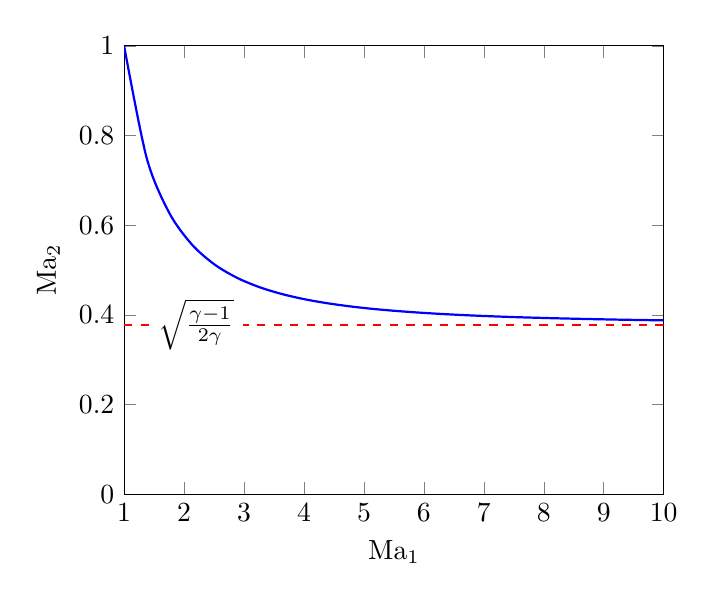
\begin{tikzpicture}
    \begin{axis}[
      xmin=1, xmax=10,
      ymin=0, ymax=1,
      ytick distance = 0.2,
      xtick distance = 1,
      xlabel={$\mathrm{Ma}_{1}$},
      ylabel={$\mathrm{Ma}_{2}$},
      ]
      \addplot[domain=1:10,smooth,thick,blue] {((2+0.4*x^2)/(2.8*x^2-0.4))^0.5};
      \addplot[domain=1:10,smooth,thick,dashed,red] {0.378};
      \node[anchor=center,fill=white] at (2.2,0.378) {$\sqrt{\frac{\gamma-1}{2\gamma}}$};
    \end{axis}
  \end{tikzpicture}
}
  \end{center}
}
\end{frame}

\begin{frame}{$\mathrm{Ma}$或$M_{*}$表示的密度比}
  \begin{itemize}
    \item \color{blue}速度比
  \end{itemize}
 \begin{equation*}
   \frac{v_{1}}{v_{2}}
   =
   \frac{v_{1}^{2}}{v_{1}v_{2}}
   =
   \frac{v_{1}^{2}}{c_{cr}^{2}}
   =
   {M_{*}}_{1}^{2}
   =
   \frac{(\gamma+1)\mathrm{Ma}_{1}^{2}}{2+(\gamma-1)\mathrm{Ma}_{1}^{2}}
 \end{equation*} 
 \uncover<2->{
 连续性方程
 \begin{equation*}
   \rho_{1}v_{1}=\rho_{2}v_{2} 
 \end{equation*}
 }
 \uncover<3->{
  \begin{itemize}
    \item \color{blue}密度比
  \end{itemize}
 \begin{equation*}
   \frac{\rho_{2}}{\rho_{1}}
   =
   \frac{v_{1}}{v_{2}}
   =
   \frac{(\gamma+1)\mathrm{Ma}_{1}^{2}}{2+(\gamma-1)\mathrm{Ma}_{1}^{2}}
 \end{equation*}
 }
\end{frame}

\begin{frame}{$\mathrm{Ma}$或$M_{*}$表示的压强比}
 \uncover<2->{
 动量方程
 \begin{equation*}
   p_{1}-p_{2}
   =
   \rho_{1}v_{2}(v_{2}-v_{1})
 \end{equation*}
 }
 \uncover<3->{
   \vspace*{-0.5em}
 \begin{equation*}
   \frac{p_{2}}{p_{1}}
   \uncover<3->{
     =
   1+\frac{\rho v_{1}}{p_{1}}(v_{1}-v_{2})
 }
 \uncover<4->{
   =
   1+\frac{\gamma v_{1}^{2}}{c_{1}^{2}}\left(1-\frac{v_{2}}{v_{1}}\right)
 }
 \uncover<5->{
   =
   1+\gamma \mathrm{Ma}_{1}^{2}\left(1-\frac{v_{2}}{v_{1}}\right)
 }
 \end{equation*}
 }
 \uncover<6->{
 \begin{equation*}
   \frac{v_{1}}{v_{2}}
   =
   {M_{*}}_{1}^{2}
   =
   \frac{(\gamma+1)\mathrm{Ma}_{1}^{2}}{2+(\gamma-1)\mathrm{Ma}_{1}^{2}}
 \end{equation*} 
 }
 \uncover<7->{
  \begin{itemize}
    \item \color{blue}压强比
  \end{itemize}
 \begin{equation*}
   \begin{aligned}
   \frac{p_{2}}{p_{1}}
   \only<7-9>{
   &=
   1+\gamma\mathrm{Ma}_{1}^{2}
   \left[1-\frac{2+(\gamma-1)\mathrm{Ma}_{1}^{2}}{(\gamma+1)\mathrm{Ma}_{1}^{2}}\right]
   \\
 }
 \only<8-9>{
   &=
   1+\frac{\gamma\mathrm{Ma}_{1}^{2}}{(\gamma+1)\mathrm{Ma}_{1}^{2}}
   (2\mathrm{Ma}_{1}^{2}-2)
   \\
 }
 \uncover<9->{
   &=
   \frac{2\gamma}{\gamma+1}\mathrm{Ma}_{1}^{2}
   -
   \frac{\gamma-1}{\gamma+1}
   \\
 }
 \uncover<11->{
   &=
   \frac{(\gamma+1){M_{*}}_{1}^{2}-(\gamma-1)}{(\gamma+1)-(\gamma-1){M_{*}}_{1}^{2}}
 }
   \end{aligned}
 \end{equation*} 
 }
\end{frame}

\begin{frame}{$\mathrm{Ma}$或$M_{*}$表示的参数比}
  \vspace*{-1em}
\begin{equation*}
   \frac{\rho_{2}}{\rho_{1}}
   =
   \frac{1}{{M_{*}}_{1}^{2}}
   =
   \frac{(\gamma+1)\mathrm{Ma}_{1}^{2}}{2+(\gamma-1)\mathrm{Ma}_{1}^{2}}
 \end{equation*}
\begin{equation*}
   \frac{p_{2}}{p_{1}}
   =
   \frac{(\gamma+1){M_{*}}_{1}^{2}-(\gamma-1)}{(\gamma+1)-(\gamma-1){M_{*}}_{1}^{2}}
   =
   \frac{2\gamma}{\gamma+1}\mathrm{Ma}_{1}^{2}
   -
   \frac{\gamma-1}{\gamma+1}
 \end{equation*}
  \begin{equation*}
    \begin{aligned}
    \frac{T_{2}}{T_{1}}
    &=
    \frac{1}{{M_{*}}_{1}^{2}}
    \frac{(\gamma+1){M_{*}}_{1}^{2}-(\gamma-1)}{(\gamma+1)-(\gamma-1){M_{*}}_{1}^{2}}
    \\
    &=
    \frac{2+(\gamma+1)\mathrm{Ma}_{1}^{2}}{(\gamma+1)\mathrm{Ma}_{1}^{2}}
    \left(
   \frac{2\gamma}{\gamma+1}\mathrm{Ma}_{1}^{2}
   -
   \frac{\gamma-1}{\gamma+1}
    \right)
    \end{aligned}
  \end{equation*}
  \begin{equation*}
    \begin{aligned}
    \frac{{p_{0}}_{2}}{{p_{0}}_{1}}
    &=
    ({M_{*}}_{1}^{2})^{\frac{\gamma}{\gamma-1}}
    \left[\frac{(\gamma+1)-(\gamma-1){M_{*}}_{1}^{2}}{(\gamma+1){M_{*}}_{1}^{2}-(\gamma-1)}\right]^{\frac{1}{\gamma-1}}
    \\
    &=
    \left[\frac{(\gamma+1)\mathrm{Ma}_{1}^{2}}{2+(\gamma-1)\mathrm{Ma}_{1}^{2}} \right]^{\frac{\gamma}{\gamma-1}}
    \left(\frac{2\gamma}{\gamma+1}\mathrm{Ma}_{1}^{2}-\frac{\gamma-1}{\gamma+1}\right)^{-\frac{\gamma}{\gamma-1}}
    \end{aligned}
  \end{equation*}
\end{frame}

\subsection{正激波在静止流体中的传播}
\begin{frame}{正激波在静止流体中的传播}
  \vspace*{-1em}
\begin{center}
  \begin{tikzpicture}
\begin{scope}
    \draw[thick] (0,0) -- (5,0);
    \draw[thick] (0,1.5) -- (5,1.5);
    %\draw[thick] (2,0) node[anchor=north]{$n$} -- (2,1.5) node[anchor=south]{$m$};
    \filldraw[thick,pattern=north east lines] (2.6,0) -- (2.6,1.5) -- (2.4,1.5)
      -- (2.4, 0) -- cycle;
    \draw[thick,-latex] (2.5,0.75) -- node[midway,above]{$v_{s}$} node[midway,below]{$p_{1}$}(3.5,0.75);
    \draw[thick,-latex] (1.0,0.75) -- node[midway,above]{$v_{g}$}
      node[midway,below]{$p_{2}$} (2.2,0.75);
    \foreach \p in 
    {0.1, 0.2, 0.3, 0.4, 0.5, 0.6, 0.7, 0.8, 0.9, 1.0,
     1.1, 1.2, 1.3, 1.4, 1.5, 1.6, 1.7, 1.8, 1.9, 2.0,
     2.1, 2.2, 2.3, 2.4, 2.5, 2.6, 2.7, 2.8, 2.9, 3.0,
     3.1, 3.2, 3.3, 3.4, 3.5, 3.6, 3.7, 3.8, 3.9, 4.0,
     4.1, 4.2, 4.3, 4.4, 4.5, 4.6, 4.7, 4.8, 4.9}
    {
      \draw[thin] (\p, 0) -- ++(-45:0.1);
      \draw[thin] (\p, 1.5) -- ++(45:0.1);
    }
  \end{scope}
  \begin{scope}[xshift=6cm]
    \draw[thick] (0,0) -- (5,0);
    \draw[thick] (0,1.5) -- (5,1.5);
    %\draw[thick] (2,0) node[anchor=north]{$n$} -- (2,1.5) node[anchor=south]{$m$};
    \filldraw[thick,pattern=north east lines] (2.6,0) -- (2.6,1.5) -- (2.4,1.5)
      -- (2.4, 0) -- cycle;
    \draw[dashed,thick] (2.3,0) node[below,anchor=north]{$2$} -- (2.3,1.5)
      node[above,anchor=south]{$2$};
    \draw[dashed,thick] (2.7,0) node[below,anchor=north]{$1$} -- (2.7,1.5)
      node[above,anchor=south]{$1$};
    \draw[thick,-latex] (2.0,0.75) -- node[midway,above]{$v_{2}=v_{s}-v_{g}$} node[midway,below]{$p_{2}$} (0.2,0.75);
    \draw[thick,-latex] (4.8,0.75) -- node[midway,above]{$v_{1}=v_{s}$} node[midway,below]{$p_{1}$}(3.0,0.75);
    \foreach \p in 
    {0.1, 0.2, 0.3, 0.4, 0.5, 0.6, 0.7, 0.8, 0.9, 1.0,
     1.1, 1.2, 1.3, 1.4, 1.5, 1.6, 1.7, 1.8, 1.9, 2.0,
     2.1, 2.2, 2.3, 2.4, 2.5, 2.6, 2.7, 2.8, 2.9, 3.0,
     3.1, 3.2, 3.3, 3.4, 3.5, 3.6, 3.7, 3.8, 3.9, 4.0,
     4.1, 4.2, 4.3, 4.4, 4.5, 4.6, 4.7, 4.8, 4.9}
    {
      \draw[thin] (\p, 0) -- ++(-45:0.1);
      \draw[thin] (\p, 1.5) -- ++(45:0.1);
    }
  \end{scope}
  \end{tikzpicture}
  \end{center}
  %在静止坐标中,激波波前气体处于静止状态,激波以速度$v_{s}$由左向右传播,激波波
  %后的气体以速度$v_{g}$也由左向右运动,其大小为分别为:
  %\begin{equation*}
    %v_{s} = v_{1},\quad v_{g}=v_{s}-v_{2}
  %\end{equation*}
\only<2-3>{ 
\begin{equation*}
   \frac{p_{2}}{p_{1}}
   =
   \frac{2\gamma}{\gamma+1}\mathrm{Ma}_{1}^{2}
   -
   \frac{\gamma-1}{\gamma+1}
   =
   \frac{2\gamma}{\gamma+1}\left(\frac{v_{1}}{c_{1}}\right)^{2}
   -
   \frac{\gamma-1}{\gamma+1}
\end{equation*}
}
\uncover<3->{
  \begin{equation*}
    v_{s} = v_{1}
    =
    c_{1}\sqrt{\frac{\gamma-1}{2\gamma}+\frac{\gamma+1}{2\gamma}\frac{p_{2}}{p_{1}}}
\end{equation*}}
\uncover<4->{
  \begin{equation*}
    v_{g}
    \only<4>{
    =
    v_{1} - v_{2}
    =
    \left(1-\frac{v_{2}}{v_{1}}\right)v_{1}
    =
    \left(1-\frac{\rho_{1}}{\rho_{2}}\right)v_{1}
  }
  \uncover<5->{
    =
    \left[1-
      \dfrac{\dfrac{\gamma+1}{\gamma-1}+\dfrac{p_{2}}{p_{1}}}
      {\dfrac{\gamma+1}{\gamma-1}\dfrac{p_{2}}{p_{1}}+1}
    \right]
    c_{1}\sqrt{\frac{\gamma-1}{2\gamma}+\frac{\gamma+1}{2\gamma}\frac{p_{2}}{p_{1}}}
    =
    \dfrac{\sqrt{\dfrac{2}{\gamma}}\left(\dfrac{p_{2}}{p_{1}}-1\right)c_{1}}
    {\sqrt{(\gamma-1)+(\gamma+1)\dfrac{p_{2}}{p_{1}}}}
  }
  \end{equation*}
}
\end{frame}

\begin{frame}{举例}
  \vspace*{-1em}
  \begin{block}
    {
      在长管中,用活塞压缩气体产生正激波。已知长管中激波前静止气体的压强
      $p_{1}=1.162\times10^{5}\mathrm{Pa}$,温度$T_{1}=292\mathrm{K}$,激波后气
      体的压强$p_{2}=1.281\times10^{5}\mathrm{Pa}$。试求激波后气体的密度
      $\rho_{2}$、温度$T_{2}$、声速$c_{2}$以及激波传播速度$v_{s}$、波后气流速度
      $v_{g}$。设气体为空气,$\gamma=1.4$,$R=287\mathrm{J/(kg\cdot K)}$。
    }
    \only<1>{
    解:激波前后气体的压强比:$
    \displaystyle
     \frac{p_{2}}{p_{1}}
     =
     \frac{1.281}{1.162}
     =
     1.102
     $
   \begin{equation*}
     \rho_{1}=
     \frac{p_{1}}{RT_{1}}
     =
     \frac{1.162\times10^{5}}{287\times292}
     =
     1.387\mathrm{kg/m^{3}}
   \end{equation*}
   \begin{equation*}
     \frac{\rho_{2}}{\rho_{1}}
     =
      \dfrac
      {\dfrac{\gamma+1}{\gamma-1}\dfrac{p_{2}}{p_{1}}+1}
      {\dfrac{\gamma+1}{\gamma-1}+\dfrac{p_{2}}{p_{1}}}
      =
      \dfrac
      {\dfrac{1.4+1}{1.4-1}\times1.102+1}
      {\dfrac{1.4+1}{1.4-1}+1.102}
      =
      1.072
      \quad
     \rho_{2}
     =
     1.486\mathrm{kg/m^{3}}
   \end{equation*}}
 \only<2>{
  \begin{equation*}
   \frac{T_{2}}{T_{1}}
   =
   \dfrac
   {\dfrac{\gamma+1}{\gamma-1}\dfrac{p_{2}}{p_{1}}+\left(\dfrac{p_{2}}{p_{1}}\right)^{2}}
   {\dfrac{\gamma+1}{\gamma-1}\dfrac{p_{2}}{p_{1}}+1}
   =
   \dfrac
   {\dfrac{1.4+1}{1.4-1}\times1.102+1.102^{2}}
   {\dfrac{1.4+1}{1.4-1}\times1.102+1}
   =
   1.028
  \end{equation*}
  \begin{equation*}
    T_{2}=1.028\times292=300.2\mathrm{K}
  \end{equation*}
  \begin{equation*}
    c_{1}=\sqrt{\gamma RT_{1}} = \sqrt{1.4\times287\times292}=342.5\mathrm{m/s}
  \end{equation*}
  \begin{equation*}
    c_{2}=\sqrt{\gamma RT_{2}} = \sqrt{1.4\times287\times300.2}=347.3\mathrm{m/s}
  \end{equation*}}
 \only<3>{
\vspace*{-1.2em}
  \begin{equation*}
    v_{s}
    =
    c_{1}\sqrt{\frac{\gamma-1}{2\gamma}+\frac{\gamma+1}{2\gamma}\frac{p_{2}}{p_{1}}}
    =
    342.5
    \sqrt{\frac{1.4-1}{2\times1.4}+\frac{1.4+1}{2\times1.4}1.102}
    =
    357.2\mathrm{m/s}
\end{equation*}
\begin{equation*}
  v_{g}
    =
    \dfrac
    {\sqrt{\dfrac{2}{\gamma}}\left(\dfrac{p_{2}}{p_{1}}-1\right)c_{1}}
    {\sqrt{(\gamma-1)+(\gamma+1)\dfrac{p_{2}}{p_{1}}}}
    =
    \dfrac
    {\sqrt{\dfrac{2}{1.4}}(1.102-1)342.5}
    {\sqrt{(1.4-1)+(1.4+1)1.102}}
    =
    23.93\mathrm{m/s}
\end{equation*}
\vspace*{-1.2em}
   \begin{itemize}
     \item $v_{1}=v_{s}>c_{1}$,$v_{2}=v_{s}-v_{g}=333.27<c_{2}$
     \item 活塞只需以速度$v_{g}=23.93\mathrm{m/s}$向前推进,即可维持强度为1.102的激波,并不需要将活塞以超声速的推进速度前进
   \end{itemize}
 }
  \end{block}
\end{frame}
